\documentclass[border=2pt]{standalone}
\usepackage[T1]{fontenc}
\usepackage{mathptmx}
\usepackage{xcolor}
\usepackage{tikz}
\usetikzlibrary{positioning,arrows.meta,fit,calc,shapes.geometric}
\definecolor{oursblue}{HTML}{0F4D92}
\definecolor{genc}{HTML}{767676}
\definecolor{fakc}{HTML}{B64342}
\definecolor{gradc}{HTML}{42949E}
\newcommand{\ffpp}{FF\texttt{++}}
\begin{document}
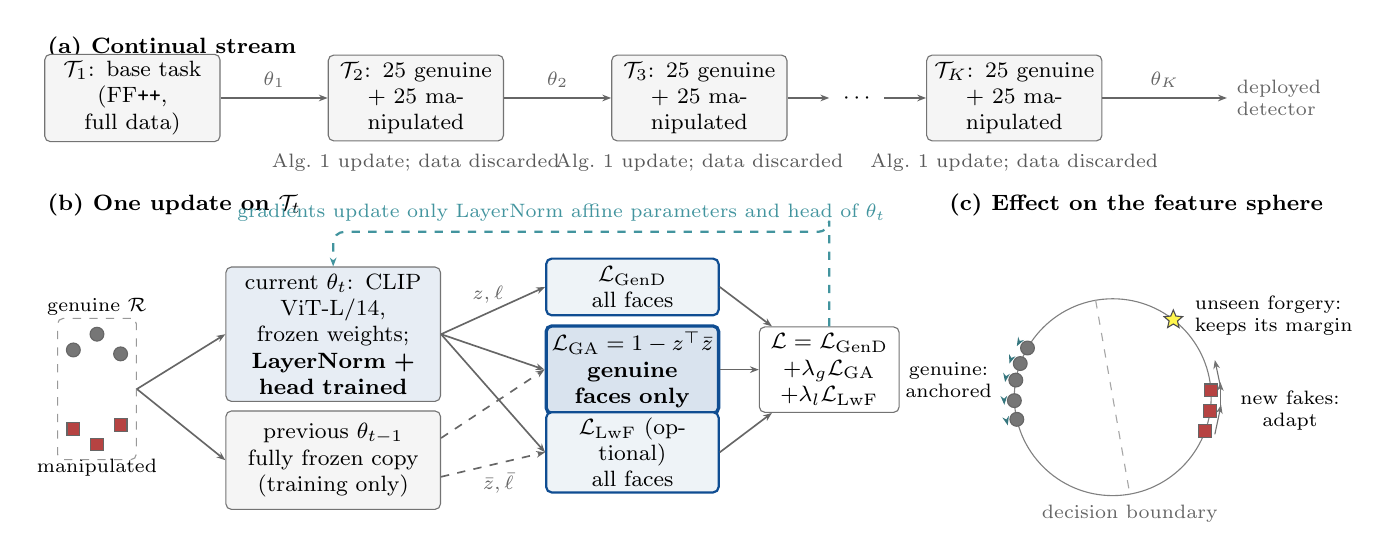
\begin{tikzpicture}[
  font=\footnotesize,
  >={Stealth[length=3.2pt]},
  box/.style={draw=black!55, rounded corners=2pt, align=center, inner sep=2.5pt},
  task/.style={box, fill=black!4, minimum height=0.85cm, text width=2.05cm},
  model/.style={box, minimum height=1.25cm, text width=2.55cm},
  loss/.style={draw=oursblue, thick, rounded corners=2pt, align=center, fill=oursblue!7, inner sep=2pt, minimum height=0.72cm, text width=2.05cm},
  gen/.style={circle, draw=black!60, fill=genc, inner sep=0pt, minimum size=5pt},
  fak/.style={rectangle, draw=black!60, fill=fakc, inner sep=0pt, minimum size=4.6pt},
  arr/.style={->, black!60, semithick},
  pan/.style={font=\footnotesize\bfseries, anchor=north west}]
% ---------------- (a) stream
\node[pan] at (-0.2,5.45) {(a) Continual stream};
\node[task] (t1) at (1.0,4.55) {$\mathcal{T}_1$: base task\\(\ffpp{}, full data)};
\node[task] (t2) at (4.6,4.55) {$\mathcal{T}_2$: 25 genuine\\+ 25 manipulated};
\node[task] (t3) at (8.2,4.55) {$\mathcal{T}_3$: 25 genuine\\+ 25 manipulated};
\node[task] (tk) at (12.2,4.55) {$\mathcal{T}_K$: 25 genuine\\+ 25 manipulated};
\node at (10.2,4.55) {$\cdots$};
\draw[arr] (t1) -- node[above, font=\scriptsize]{$\theta_1$} (t2);
\draw[arr] (t2) -- node[above, font=\scriptsize]{$\theta_2$} (t3);
\draw[arr] (t3) -- (9.85,4.55); \draw[arr] (10.55,4.55) -- (tk);
\draw[arr] (tk) -- node[above, font=\scriptsize]{$\theta_K$} (14.9,4.55) node[right, align=left, font=\scriptsize]{deployed\\detector};
\foreach \t in {t2,t3,tk} \node[font=\scriptsize, text=black!65, below=1pt of \t] {Alg.~1 update; data discarded};
% ---------------- (b) one update
\node[pan] at (-0.2,3.45) {(b) One update on $\mathcal{T}_t$};
\node[gen] (g1) at (0.25,1.35) {}; \node[gen] (g2) at (0.55,1.55) {}; \node[gen] (g3) at (0.85,1.3) {};
\node[fak] (f1) at (0.25,0.35) {}; \node[fak] (f2) at (0.55,0.15) {}; \node[fak] (f3) at (0.85,0.4) {};
\node[font=\scriptsize, align=center] at (0.55,1.9) {genuine $\mathcal{R}$};
\node[font=\scriptsize, align=center] at (0.55,-0.15) {manipulated};
\node[draw=black!40, dashed, rounded corners=2pt, fit=(g1)(g2)(g3)(f1)(f2)(f3), inner sep=3pt] (batch) {};
\node[model, fill=oursblue!10] (cur) at (3.55,1.55) {current $\theta_t$: CLIP\\ViT-L/14, frozen weights;\\\textbf{LayerNorm + head trained}};
\node[model, fill=black!4] (prev) at (3.55,-0.05) {previous $\theta_{t-1}$\\fully frozen copy\\(training only)};
\draw[arr] (batch.east) -- (cur.west);
\draw[arr] (batch.east) -- (prev.west);
\node[loss] (lgend) at (7.35,2.15) {$\mathcal{L}_{\mathrm{GenD}}$\\all faces};
\node[loss, very thick, fill=oursblue!16] (lga) at (7.35,1.1) {$\mathcal{L}_{\mathrm{GA}}=1-z^{\top}\bar z$\\\textbf{genuine faces only}};
\node[loss] (llwf) at (7.35,0.05) {$\mathcal{L}_{\mathrm{LwF}}$ (optional)\\all faces};
\draw[arr] (cur.east) -- node[above, font=\scriptsize, pos=0.45]{$z,\ell$} (lgend.west);
\draw[arr] (cur.east) -- (lga.west);
\draw[arr] (cur.east) -- (llwf.west);
\draw[arr, dashed] ([yshift=8pt]prev.east) -- (lga.west);
\draw[arr, dashed] ([yshift=-6pt]prev.east) -- node[below, font=\scriptsize, pos=0.55]{$\bar z,\bar\ell$} (llwf.west);
\node[box, fill=white, text width=1.6cm] (sum) at (9.85,1.1) {$\mathcal{L}=\mathcal{L}_{\mathrm{GenD}}$\\$+\lambda_g\mathcal{L}_{\mathrm{GA}}$\\$+\lambda_l\mathcal{L}_{\mathrm{LwF}}$};
\draw[arr] (lgend.east) -- (sum); \draw[arr] (lga.east) -- (sum); \draw[arr] (llwf.east) -- (sum);
\draw[->, thick, gradc, dashed, rounded corners=4pt] (sum.north) |- (9.85,2.85) -| node[pos=0.27, above, font=\scriptsize, text=gradc]{gradients update only LayerNorm affine parameters and head of $\theta_t$} (cur.north);
% ---------------- (c) hypersphere intuition
\node[pan] at (11.25,3.45) {(c) Effect on the feature sphere};
\def\R{1.25}
\coordinate (O) at (13.45,0.75);
\draw[black!50] (O) circle (\R);
\draw[black!35, dashed] ($(O)+(100:\R)$) -- ($(O)+(280:\R)$);
\node[font=\scriptsize, text=black!60, anchor=north] at ($(O)+(280:\R)+(0,-0.02)$) {decision boundary};
% genuine cluster: anchored (tiny moves)
\foreach \a in {150,160,170,182,193} {
  \node[gen] at ($(O)+(\a:\R)$) {};
  \draw[->, gradc!80!black, thin] ($(O)+(\a:\R)+(\a:0.13)$) -- ($(O)+(\a+2:\R)+(\a+2:0.13)$);
}
\node[font=\scriptsize, align=center, anchor=east] at ($(O)+(170:\R)+(-0.18,0)$) {genuine:\\anchored};
% stream fakes: free to move
\foreach \a in {-20,-8,4} {
  \node[fak] at ($(O)+(\a:\R)$) {};
  \draw[->, black!55, thin] ($(O)+(\a:\R)+(\a:0.13)$) -- ($(O)+(\a+16:\R)+(\a+16:0.13)$);
}
\node[font=\scriptsize, align=center, anchor=west] at ($(O)+(-8:\R)+(0.26,0)$) {new fakes:\\adapt};
% unseen fake keeps its margin
\node[star, star points=5, star point ratio=2.2, draw=black!70, fill=yellow!70, inner sep=0pt, minimum size=7pt] at ($(O)+(52:\R)$) {};
\node[font=\scriptsize, align=left, anchor=west] at ($(O)+(52:\R)+(0.15,0.05)$) {unseen forgery:\\keeps its margin};
\end{tikzpicture}

\end{document}
